% !TeX program = lualatex
\begin{filecontents*}{\jobname-url.mst}
% Input style specifiers
keyword "\\urlentry"
% Output style specifiers
preamble "\\begin{theurls}"
postamble "\\end{theurls}\n"
group_skip ""
headings_flag 0  
item_0 "\n\\urlitem{"
delim_0 "}{"
delim_t "}"
line_max 500
\end{filecontents*}

\RequirePackage{scrlfile}
\AfterClass{article}{
  \RequirePackage[hyphens,spaces,obeyspaces]{url}
}
\documentclass[
	english,
	twocolumn,
	marginpar=false,
	papersize=a4paper,
	accentcolor=9c,
    IMRAD=false,
	]{tudapub}

\usepackage{etoolbox}

%\AtEndPreamble{\hypersetup{breaklinks}}

\usepackage[english]{babel}
\usepackage[babel]{csquotes}
\usepackage{caption} % https://en.wikibooks.org/wiki/LaTeX/Labels_and_Cross-referencing#Issues_with_links_to_tables_and_figures_handled_by_hyperref
\usepackage{fancyvrb}
\usepackage{varwidth}
\usepackage{hologo}
\usepackage{amssymb}
\usepackage[backend=biber,style=numeric,sorting=ynt]{biblatex}
\usepackage{hyperref}
\usepackage[toc,acronym,automake=immediate]{glossaries}
%\usepackage[undefaction=warn]{glossaries-extra}
\usepackage[most]{tcolorbox}
\usepackage[official]{eurosym}
\usepackage{graphicx}
\usepackage{csquotes}
\usepackage{xcolor}
\usepackage{listings}

% allow better line breaks in URLs
\gappto{\UrlBreaks}{\do\_}
\gappto{\UrlBreaks}{\UrlOrds}

% colorbox
\newtcolorbox{myframe}[1][]{
  enhanced,
  arc=0pt,
  outer arc=0pt,
  colback=TUDa-9c,
  boxrule=0.8pt,
  #1
}

% listings
\lstdefinestyle{BashInputStyle}{
  language=bash,
  basicstyle=\small\sffamily,
  numbers=left,
  numberstyle=\tiny,
  numbersep=3pt,
  frame=tb,
  columns=fullflexible,
  backgroundcolor=\color{yellow!10},
  linewidth=0.9\linewidth,
  xleftmargin=0.1\linewidth
}

% glossary
% glossary
\makeglossaries

\newacronym
  {ash}{ASH}{\gls{ASH}}
\newacronym
  [description={\textit{\acrlong{ccitt}} – Advisory committee to the International Telecommunication Union}]
  {ccitt}{CCITT}{Comité Consultatif International Télégraphique et Téléphonique}
\newacronym
  [description={\textit{\acrlong{cpm}}, an early operating system}]
  {cpm}{CP/M}{Control Program for Microcomputers}
\newacronym
  [description={\textit{\acrlong{cpu}} of a computer system}]
  {cpu}{CPU}{Central Processing Unit}
\newacronym
  [description={\textit{\acrlong{crt}}: technology for building computer screens}]
  {crt}{CRT}{cathode ray tube}
\newacronym
  {dtp}{DTP}{\gls{DTP}}
\newacronym
  [description={A \textit{\acrlong{four-cc}} used as an identifier for a file format or sub-structure}]
  {four-cc}{FourCC}{four character code}
\newacronym
  [description={\gls{IANA}}]
  {iana}{IANA}{Internet Assigned Numbers Authority}
\newacronym
  [description={\textit{\acrlong{iff}}: Precursor to \acrshort{tiff}}]
  {iff}{IFF}{Image File Format}
\newacronym
  [description={\textit{\acrlong{isa}}: The format and semantics of the machine code that a \acrshort{cpu} executes}]
  {isa}{ISA}{instruction set architecture}
\newacronym
  {html}{HTML}{hyper text markup language}
\newacronym
  {m68k}{m68k}{Motorola 68000 line of chips}
\newacronym
  {midi}{MIDI}{Musical Instrument Digital Interface}
\newacronym
  {mime}{MIME}{Multipurpose Internet Mail Extensions}
\newacronym
  {os}{OS}{Operating System}
\newacronym
  {pdf}{PDF}{portable document format}
\newacronym
  {pdl}{PDL}{page description language}
\newacronym
  {png}{PNG}{portable network graphic}
\newacronym
  {ps}{PS}{Adobe PostScript}
\newacronym
  [description={\textit{\acrlong{rom}}: Usually used to build software for an operating system or firmware for a device into a computer.}]
  {rom}{ROM}{read only memory}
\newacronym
  {rtf}{RTF}{rich text format}
\newacronym
  [description={\textit{\acrlong{tiff}}: Container format for images}]
  {tiff}{TIFF}{Tagged Image File Format}
\newacronym
  {tos}{TOS}{The Operating System}
\newacronym
  [description={\textit{\acrlong{wysiwyg}} – A kind of editor that shows the visual output of what is currently being edited}]
  {wysiwyg}{WYSIWYG}{''What You See Is What You Get''}

\newglossaryentry{accessory}
  {name=accessory, plural=accessories, description={Loadable extension to the GEM Disk Operating System}}
\newglossaryentry{ATARI}
  {name={ATARI}, description={\textit{Atari, Inc.} – US-American computer manufacturer and games publisher}}
\newglossaryentry{bit}
  {name={bit}, description={Fundamental unit in computing. Value that is either $0$ or $1$, off or on, false of true, unset or set}}
\newglossaryentry{byte}
  {name={byte}, description={Fundamental unit in computing. A byte is made up of 8 bits and can represent $256$ different values}}
\newglossaryentry{ASH}
  {name={Application Systems /// Heidelberg}, description={Software and Games Publisher based in Heidelberg, Germany. Publisher of Signum! and \textit{Das Signum! Buch}}}
\newglossaryentry{charset}
  {name=charset, description={A collection of glyphs mapped to keys, much like a font but explicitly including other uses like box drawing characters}}
\newglossaryentry{codepoint}
  {name=codepoint, description={Unique number assigned to a character or ligature by the Unicode Standard}}
\newglossaryentry{DRI}
  {name={Digital Research, Inc.}, description={A company founded by Gary Kildall}}
\newglossaryentry{DTP}
  {name={desktop publishing}, description={The process of preparing documents with a computer system}}
\newglossaryentry{encoding}
  {name=encoding, description={A mapping between a sequence of bytes and a sequence of characters}}
\newglossaryentry{hardcopy}
  {name=Hardcopy, description={A term used to describe the process of printing the current content of the computer screen. Roughly equivalent to the modern term \textit{screenshot}. See also: \url{https://www.stcarchiv.de/tos1991/02/hardcopies-mit-mr-print}}}
\newglossaryentry{Header}
  {name={Header}, description={Metadata associated with a document or message that is usually stored at the start or end}}
\newglossaryentry{IANA}
  {name={Internet Assigned Numbers Authority}, description={The standards body in charge of maintaining registries of names and numeric identifiers for internet protocols}}
\newglossaryentry{IFF}
  {name={IFF}, description={Image File Format}}
\newglossaryentry{Media Type}
  {name={Media Type}, description={Also known as MIME type; unique identifier for a file format registered with the IANA}}
\newglossaryentry{Signum!2}
  {name={Signum!2}, description={Second edition of the Signum! word processor and main subject of this paper}}
\newglossaryentry{Unicode}
  {name={Unicode}, description={Standard that is published by the consortium of the same name with the goal of unifying text encoding across all languages}}
\newglossaryentry{word}
  {name={word}, description={Fundamental unit in computing. Describes the default size of memory depending on the processor architecture. For the ATARI, a WORD is 2 bytes or 16 bits}}
\usepackage{pdfescape}
\usepackage{xstring}

% https://tex.stackexchange.com/questions/121977/auto-generate-list-of-url-usages-within-document

\makeatletter
\newwrite\file@url
\openout\file@url=\jobname-url.idx\relax

\newcommand*{\write@url}[1]{%
  \begingroup
    \EdefEscapeHex\@tmp{#1}%
    \protected@write\file@url{}{%
      \protect\urlentry{\@tmp}{\thepage}%
    }%
  \endgroup
}
\let\saved@hyper@linkurl\hyper@linkurl
\renewcommand*{\hyper@linkurl}[2]{%
  \write@url{#2}%
  \saved@hyper@linkurl{#1}{#2}%
}
\newcommand*{\listurlname}{List of URLs}
\newcommand*{\printurls}{%
  \InputIfFileExists{\jobname-url.ind}{}{}%
}
\newenvironment{theurls}{%
  \section*{\listurlname}%
  \@mkboth{\listurlname}{\listurlname}%
  \let\write@url\@gobble  
  \ttfamily
  \raggedright
  \setlength{\parfillskip}{0pt}%
}{%
  \par
}
\newcommand*{\urlitem}[2]{%
  \hangindent=1em
  \hangafter=1   
  \begingroup    
    \EdefUnescapeHex\@tmp{#1}%
    \expandafter\url\expandafter{\@tmp}%
  \endgroup
  \urlindex@pfill
  \IfSubStr{#2}{,}{pp}{%
    \IfSubStr{#2}{-}{pp}{p}%
  }.\@\space\ignorespaces%
  #2%
  \par
}
\newcommand*{\urlindex@pfill}{% from \pfill of package `doc'
  \unskip~\urlindex@dotfill
  \penalty500\strut\nobreak
  \urlindex@dotfil~\ignorespaces
}
\newcommand*{\urlindex@dotfill}{% from \dotfill of package `doc'
  \leaders\hbox to.6em{\hss .\hss}\hskip\z@ plus  1fill\relax
}
\newcommand*{\urlindex@dotfil}{% from \dotfil of package `doc'
  \leaders\hbox to.6em{\hss .\hss}\hfil
}
\makeatother
\immediate\write18{makeindex \jobname-url}
% https://gist.github.com/martinarroyo/b9e0a963ad27169a6eee
\newif\ifproblems
%\problemstrue % comment out to hide problems
\newcounter{problems}
\setcounter{problems}{0}

\newcommand{\problem}[2]{%
    \ifproblems
    \stepcounter{problems}%
    \fbox{%
    \color{blue}#1%
    {\color{black}: \normalfont #2}}
    \fi}

\newcommand{\citationneeded}[1]{\problem{Citation needed}{#1}}
\newcommand{\fixme}[1]{\problem{FixMe}{#1}}

\newcommand{\checkproblems}{
	\ifproblems
	\ifnum\value{problems} > 0
	\begin{center}
		You have \arabic{problems} problems(s). Bad!
	\end{center}
	\else
	No problems. Good!
	\fi
	\fi
}

% bibliography
\addbibresource{signum.bib}

% custom commands
\newcommand{\T}[1]{\texttt#1}
\newcommand{\Signum}{\textit{Signum!}}
\newcommand{\funfact}[1]{%
\footnote{%
  %{\vspace{3mm}\begin{center}
  %  \framebox[0.8\columnwidth]{%
  %    \parbox{0.75\columnwidth}{%
        \textbf{\color{TUDa-9c}Fun Fact} #1
        %{\color{black}\normalfont #1}%
  %    }%
  %  \par}
  %\end{center}}%
}}
%\vspace{3mm}}

% ----------------------------------------------------------

% TODO: Introduction, Rust, Macros

\begin{document}
%Zusätzliche Metadaten für PDF/A. In diesem Fall notwendig, weil Titel ein Makro enthält.
\Metadata{
	author=Daniel Seiler,
	title=The Signum! System,
	subject=Analysis and Reverse Engineering of a file format,
	date=2021-02-15,
	keywords=Sprachenzentrum \sep Wordprocessing \sep Atari
}

\title{Reverse-Engineering a Word-Processor: The Signum! System}
\subtitle{Analysis and re-implementation of a discontinued document file format}
\author{Daniel Seiler}

\titleimage{\includegraphics*[trim=0 630 0 300,width=\width,clip]{img/title.jpg}}

% Infoboxen
\addTitleBox{Research paper at the Sprachenzentrum}
%\addTitleBoxLogo{img/ash}
%\addTitleBoxLogo*{
\includegraphics[width=0.5\linewidth]{img/ash}}

\maketitle

\begin{abstract}
    In the 1980s, when personal computers with graphical user interfaces
    began to become common in homes and universities, there was an increasing demand to use computers to help with document preparation.
    
    Sometimes referred to as the \textit{\acrfull{dtp} revolution}, this decade saw the invention of \acrshort{dtp} technology that set the foundation for the tools we use today. This includes the initial releases of WordStar (1978), Microsoft Word (1983), PostScript (1984), \TeX{} (1986), and PDF (1993).
    
    This paper describes one of the tools of the time. The \gls{Signum!2} word processing system was a common tool used to write theses and papers in Germany in the 1980s. It was only available on the ATARI ST line of personal computers, created by mathematician Franz Schmerbeck and published by \acrfull{ash}.
    
    \Signum{} was never released for newer operating systems after the ATARI ST was discontinued. The documents that were prepared with it are not compatible with modern software and conversions to other formats are rare and incomplete. In this paper, I also present the results of my personal research into these files, the approach that I took and what I learned about the way \Signum{} works.
\end{abstract}

\tableofcontents

\section*{Introduction}
\label{sec:intro}
\addcontentsline{toc}{section}{\nameref{sec:intro}}

%\fixme{Sachlicher}
% - This is what I did
% - "Contributions"
% - Explain what Signum! is relative to ATARI
% - Why now -- missing experience 10 years ago

This paper describes my experience with extracting text documents from a discontinued computer system – from reading files off of floppy disks that were stored in my parents' basement to decoding images in an undocumented file format.

I provide a short overview over the ATARI ST line of computers, the components that it consists of and available methods to use its programs and storage devices in the present day. Then, I present the commercial \Signum{} word processing system, its motivation, mechanics and basic user interface.

Next, I present general concepts of file formats and original research into two file formats that are used by Signum. This is information that was not previously available to the public.

Finally, I provide an overview of existing methods to convert Signum documents into more modern formats, introduce my own system to convert Signum files to \acrshort{pdf} and discuss key challenges and decisions pertaining to that project.

%In August of 2020, I started to look into a box of old floppy disks from my parents' basement. These disks were originally used on an ATARI ST and later a Windows 95 machine, that are still stored in the same room.

%A few of the disks were marked with the term \textit{Signum!}. My dad told me that this was the program he used to write his masters thesis (\textit{Magister Artium}) and that the thesis itself should be on one of the disks as well.

%So, after making copies of all the floppy disks that were still in good shape, I focused on the ones that were related to Signum!. I was very excited to find files like \textbf{EINLEITU.SDO}, \textbf{MAGISTER.SDO} and \textbf{SCHLUSS.SDO} on one of the disks, but also realized that this was a custom file format with no modern tools available to read it.

%Looking at the content of the files, I noticed that much of the text was actually readable with a bit of effort (c.f. \autoref{fig:sdo-hexdump}), so started to work on a system that automated this. In this process, I learned a lot about Signum!, it's file format and also word processing, document preparation and font handling in general, which is presented in this paper.

\paragraph{Contributions} This paper offers a description of the structure of the Signum!2 document file format, a description of the associated \textit{bimc} image file format and its compression algorithm and a description of three particular challenges that arise from creating a new software that reads those files, namely character positioning, using bitmap fonts and character encoding.
\section{The ATARI ST line of personal computers}
\label{sec:atarist}

The US-American hardware and software company \gls{ATARI} started out by creating very successful video game consoles for pubs and other public spaces. At that time, hardware and software of these machines were still tightly integrated. The first game of this kind was \textbf{Pong}, a simple two-player game derived from tennis.

After that, ATARI created multiple consumer video-game consoles, which brought computer games directly into individual households. In 1979, they announced their first general purpose 8-bit computers, the \textit{400} and the \textit{800}.

In 1985, ATARI introduced their next generation of home computers: The \textbf{ATARI ST}\footnote{\url{https://archive.org/details/atarist}}. They were relatively inexpensive and achieved wide adoption on the Western European market.

The first computers of the series (260ST, 520ST, 520ST+) featured a dedicated sound chip, a \acrshort{rom} cartridge slot, \acrshort{midi} input and output ports, an external \acrshort{crt} monitor, a parallel port for a printer, a serial port for a modem, an external floppy disk drive, a connector for an external hard drive, and ports for a mouse and a joystick. The keyboard was integrated into the case of the machine. The later computers of the series (1040ST) had a floppy disk drive built in \cite{vogt2021History}.

The \acrfull{midi} ports turned the ATARI ST into a machine that was useful in music studios and other kinds of real-time digital signal processing such as experiments in physics or electrical engineering in academic settings\footnote{\url{https://archive.org/details/MIDIMusi1986}}.

The name \textbf{ST} refers to the sixteen/thirty-two \gls{bit} \acrfull{isa} of the \acrfullpl{cpu}, which were from the \acrfull{m68k}. These chips used the 16-bit \gls{word} as their fundamental unit of data storage but used 32-bit addresses for the main memory.

Similar to the \textit{Apple Lisa} computer, the ATARI ST was part of the first generation of computers to be distributed with a graphical user interface as part of the operating system. This development is ultimately derived from the 1968 ``mother of all demos'' by Douglas Engelbart. With his \textbf{oN-Line System}, Engelbart and colleagues had demonstrated the first prototype of the \textbf{WIMP} paradigm; making use of Windows, Images, Menus, and a (Mouse)Pointer \cite{english1967display}.

\begin{figure}[h]
    \centering
    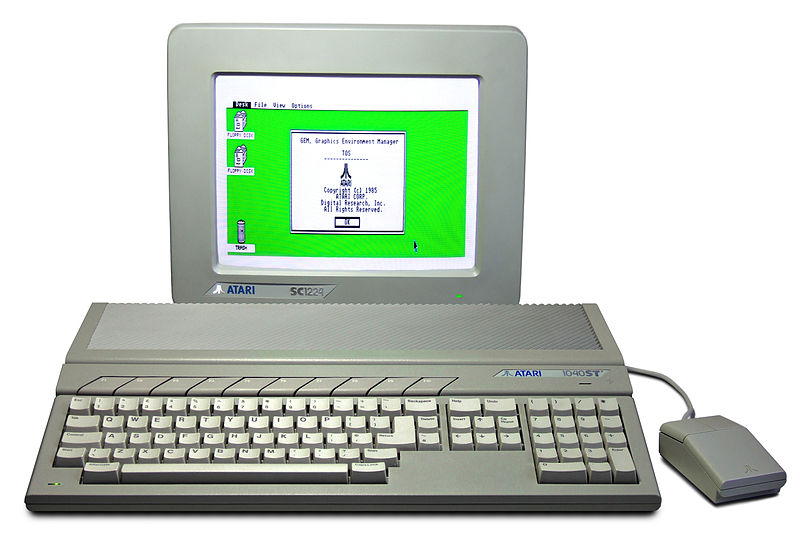
\includegraphics[width=\columnwidth]{img/800px-Atari_1040STf.jpg}
    \caption{Picture of an Atari 1040ST\textsuperscript{F}; \copyright Bill Bertram, 2006, \url{https://commons.wikimedia.org/wiki/File:Atari_1040STf.jpg}}
    \label{fig:atari_1040st}
\end{figure}

\subsection{Recovering floppy disks today}
\label{sec:floppy-disks}

%\funfact{My research into this topic started with a box of floppy disks marked Signum! in my parents' basement}
The very first versions of the ST line had neither a hard disk for persistent storage nor a built-in drive for removable media. Consumers had to buy an additional floppy disk drive to load the programs that they wanted to use and to store the data that they generated.

In those days, a consumer would insert the floppy disk for a program like \textit{Signum!}, start the program, which would load the complete program into the main memory, insert another floppy disk with the files they wanted to edit, and use the open program to work with those files.

The type of floppy disk used with the ATARI ST computers were 3.5'' (inches), with a storage capacity of about 720 kilobytes. Later advances in disk technology allowed for so-called \textit{double-density} disks with about 1.4 megabytes in storage space.

To analyze or recover documents created with the \Signum{} word processor, it's very likely that we need to read such disks because that is where files were saved at the time. As modern computers do not have a floppy disk drive anymore, the first step is to acquire an external drive that can be connected via USB cable. This enables me to make a complete copy of the disk that we can work on without putting any more strain on the original physical disk.

I used the \texttt{ddrescue} command line tool available for the Linux operating system to perform that recovery. The result is single image file per disc; the conventional file extensions for these images is \textit{*.st} \cite{archiveteam:stdisc}.

\begin{lstlisting}[style=BashInputStyle]
$ ddrescue -n /dev/sdb myfloppy.st myfloppy.log
\end{lstlisting}

As with modern disks or flash drives, an ST-compatible floppy disk consists of a hierarchy of files and folders. To that end, the disk image is structured according to a file-system, in this case \textbf{FAT12}. Fortunately, the FAT12 file system is not exclusive to the ST and a modern Linux system still supports it with only minor differences relating to the last-edited timestamps on the files.

Hence, I can \textit{mount} a floppy disk image into our main file-system using a simple \texttt{mount} command, provided the directory \texttt{/mnt/floppy} exists:

\begin{lstlisting}[style=BashInputStyle]
$ mount -ro myfloppy.st /mnt/floppy
\end{lstlisting}

I can now use the files from the floppy disk for any subsequent processing that may be necessary, without the risk of damaging the original disks.

\subsection{Using a machine emulator}
\label{sec:emulator}

One useful tool in analyzing the Signum! word processor is the ability to run the original software in a machine emulator. Emulation, in this case, refers to the simulation of the original \acrshort{m68k} \acrshort{cpu} and associated peripherals of an ST computer using software that runs on a modern computer.

Thanks to a large number of people interested in retro-computing, there are multiple emulators available for the ATARI ST as well as associated archives of software to run on these computers. 

The most important component of this setup is the \textbf{\acrshort{tos}-\acrshort{rom}}, that is the \acrlong{rom} representation of \acrlong{tos}. This piece of software was distributed as a built-in storage chip in the original ST computers so it's not really hardware that can be simulated. This is also the most problematic component of the system, because neither Atari, Inc. nor its legal successors have released the copyright to it.

However, there are a number of alternatives:
\acrlong{ash} published the \textbf{MagiC} operating system in 1992. It is a direct replacement for the original \acrshort{tos} and adds new features such as multitasking. It was later incorporated into the \textit{MagiCMac} and \textit{MagiCPC} emulators, that embeds the \acrshort{os} into a program running on Macs and PCs.
The \textbf{EmuTOS} project has also developed an alternative but compatible operating system based on the original GEMDOS sources from Digital Research, that were released under a permissive license around the year 2000 \cite{emuTOSHistory}. This system is available for free under the GPL license.

As I am using a \textit{debian GNU/Linux} system for this research, I chose the \textbf{Hatari} emulator \cite{hatari}, which is readily available as an extension package for my operating system.

Using that system, I could install a copy of \textit{Signum!2}, which is amazingly still available for purchase on the ASH website\footnote{\url{https://www.ashshop.biz/diverses/atari/textverarbeitung/874/signum-2-download}}.

\subsection{TOS - The Operating System}

The operating system of the ATARI ST computers is mostly adapted from products by \gls{DRI}, a company that created the successful \acrshort{cpm} operating system, originally designed for 8-bit microcomputers.

As detailed in \textit{The documentation for TOS}\funfact{The TOS Guide is maintained by the FreeMINT project, aiming to bring a modern operating system to ATARI-ST compatible hardware} \cite{tos.hyp}, the TOS consists of multiple components that work together to create the full operating system:

\begin{description}
    \item[GEM] This is the user-facing name of the full graphical operating system. It is the name of a product by Digital Research and presents a set of windows, icons and menus to the user, who can interact with them using a mouse.
    \item[VDI] The Virtual Device Interface is the low-level graphics system that allows a programmer to display text, images or lines on the screen.
    \item[AES] The Application Environment Services are the high-level parts of the GEM that allow a programmer to define windows and menus.
    \item[GEMDOS] The GEM Disc Operating System is the standard library of functions for a GEM program. It includes subroutines relating to loading and saving files, managing memory or processes or accessing the network.
    \item[BIOS] This Basic Input-Output System is the lower half of a standard operating system. It provides the hardware-specific subroutines that the (GEM)DOS needs to work.
    \item[XBIOS] This eXtended BIOS is a collection of subroutines that provide advanced control of the additional subsystems of the ST, such as the sound chip, the MIDI ports, the keyboard and the printer.
\end{description}

\subsection{The GEM User Interface by Digital Research Inc.}

The original GEM System allows only one application to run at any one time. An application consists of a menu bar, a main background window and a set of floating windows or dialogs.

The default application, which is launched whenever the system is started, is the Desktop or \textbf{Desk}. This application provides access and overview to the installed drives and includes a drag-and-drop file manager. To start a program such a Signum!, you would put in the appropriate floppy disk, double click on the corresponding icon on the desktop, navigate to the folder that contains the \texttt{SIGNUM2.PRG} executable and start the programm by, again, double-clicking the icon.

\begin{figure}[h]
    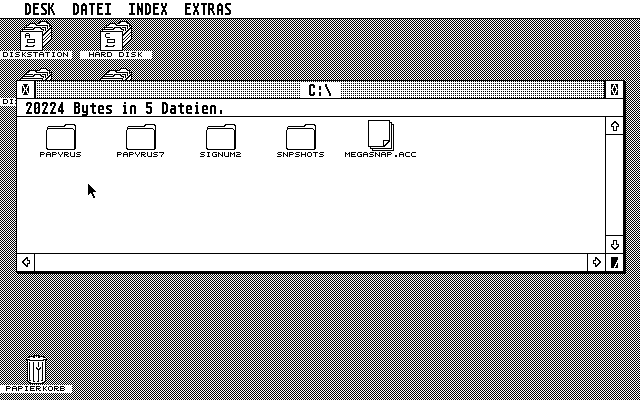
\includegraphics[width=\columnwidth]{img/SNAP2.png}
    \caption{Screenshot of the GEM Desktop Application. \textbf{MEGASNAP.ACC} is an example for an accessory. It can be used to take screenshots like this one.}
\end{figure}

There was one important exception to the rule of allowing only a single application to run at a time: So called \glspl{accessory} are programs that have a file extension of \texttt{ACC}, and which are loaded when the computer is started, provided they are stored at the root of the disk that is inserted while the computer is starting.
\section{The Signum! word processor}

The \gls{Signum!2} word processor is a computer program written by Franz Schmerbeck\footnote{\url{http://schmerbeck.de/}} for the ATARI ST in the 1980s. It was and still is being distributed by the Heidelberg-based company \gls{ASH} (ASH), which has also provided user-support. ASH furthermore published a comprehensive guide in book form \cite{ritzhaupt1988signum}.

In his foreword to \textit{Das Signum! Buch}, the author of \Signum{} explains that the program was written for all the users who were limited by the \textquote{Standard of normal word processing systems}. He ended up writing his own thesis for a mathematics degree (\textit{Diplom}) on a typewriter for lack of alternatives and explains:

\foreignblockquote{german}[{\cite[Page 7]{ritzhaupt1988signum}}]{
    %Die Idee zur Entwicklung von Signum entspringt eigenen (mühsamen) Erfahrungen im Bereich der Textverarbeitung. Sie gipfelte in der Erstellung einer Diplomarbeit in Mathematik mit einer Schreibmaschine. Jeder, der eine solche Arbeit einmal gesehen hat, weiß, was das bedeutet: Griechische Symbole und mathematische Sonderzeichen kommen fast mit der selben Häufigkeit vor wie normaler Fließtext. Dies bedeutet ein ständiges Wechseln zwischen mindestens drei verschiedenen Kugelköpfen.
    
    Tritt man aus dem Elfenbeinturm der eigenen Fakultät, so erkennt man, daß viele Textanwendungen außerhalb der Naturwissenschaften mit ähnlichen Problemen behaftet sind: Man denke z.B. an mehrsprachige Übersetzungen (griechisch, kyrillisch, hebräisch), Dokumentationen im Handel, in der Technik (grafische Sonderzeichen), oder an die anspruchsvolle Aufbereitung eines Textes (verschiedene Schriftarten und -größen). Diese Anwendungen können mit Standardsysteme oft nicht oder nur mit unzureichender Qualität bewältigt werden.
    
}

These requirements are directly reflected in the implementation of \Signum{}: Firstly, its free-form layout mode allows mathematical formulas to be typeset with minimal effort and a \acrshort{wysiwyg} user interface.

Secondly, it allows the use of up to $7$ \textit{character sets} or \glspl{charset}, which are sets of 127 glyphs that are mapped to keys on the keyboard. In the editor, a user can set one charset as the default (``\textit{Normal}''), one charset to be used while holding the \textit{Alternate} key and one charset to be used while holding the \textit{Control} key.

In addition to using \glspl{charset} to have the same font in multiple sizes, this system allows the users to add text in other writing systems such as Hebrew, Arabic or Greek or simple drawings like chemical formulas, box drawing characters, smileys with minimal overhead\funfact{There's even a charset with a \textit{cut this paper here} mark.}.

The character sets also play a crucial role in making Signum! a tool that can produce high-resolution documents while using a low-resolution graphical interface. For every device that needs to display or print these characters there is a different font file. The editor uses the low-resolution \textbf{.E24} file format while a 24-needle printer would use \textbf{.P24} files that have about 3 times the resolution. There are additional file formats for other printer types.

\begin{figure}[h]
    \centering
    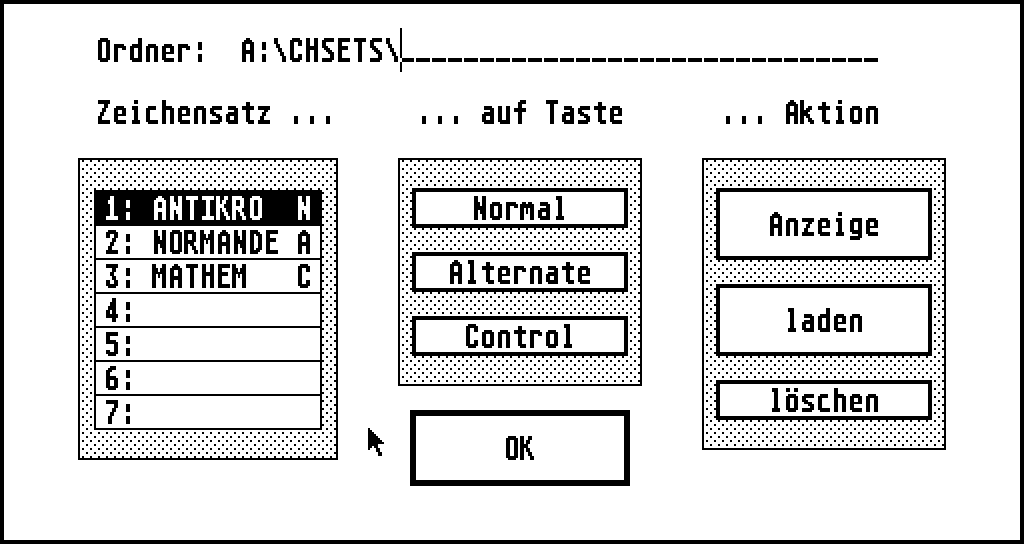
\includegraphics[width=\columnwidth]{img/cset-dialog.png}
    \caption{The character set dialog \label{fig:cset-dialog}}
\end{figure}

\subsection{Word processing with Signum!}

Given the limitations of the time, \gls{Signum!2} works very much like its modern successors. The main feature of the interface is a visual representation of a page. There is a cursor that indicates the current insertion point and when the user presses a key, the corresponding character is placed at that point and the cursor moves forward. When the cursor reaches the end of a line, it automatically moves or breaks the current word to the next line and continues from there.

A document consists of up to a hundred pages, only one of which is active at a time. The current page number is displayed in the bottom right corner of the editor. The cursor can be placed anywhere on a two by two pixel grid. The vertical component of a position in the grid is called the \textit{(micro-)line}. The value for the cursor's vertical position is also displayed in the bottom right.

There are separate header and footer areas on each page, which hold page number information and footnotes and don't interfere with breaking paragraphs across pages.

%\noindent\fixme{escape-sequences}\\
%TODO: Finally, a lot of menu commands are also available as \textit{escape-sequences}, that is sequences of key-presses that start with the \textit{escape} key. These sequences could change the position of the cursor, 

\Signum{} also has a macro system, whereby a sequence of key presses can be recorded and played back at a later point in time. This is especially useful in conjunction with the escape sequences. Escape sequences are combinations of key presses that start with \texttt{ESC} and can change settings such as the current \textit{normal} character set.

\begin{figure}
    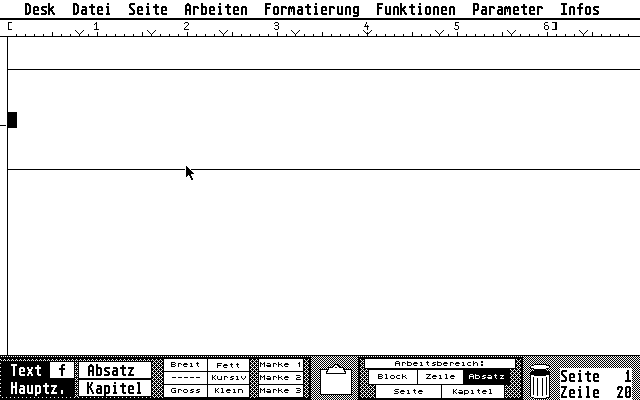
\includegraphics[width=\columnwidth]{img/SNAP3.png}
    \caption{Signum!2 immediately after starting the program. The first menu would be called \texttt{SIGNUM!} if the screenshot tool wasn't installed.}
    \label{fig:sig2_start}
\end{figure}

\subsubsection{Writing Modes}
While the grid allows for some flexibility in typesetting, the default behavior of the system guides the user to a regular page layout. In the bottom left corner of the editor, there is a set of buttons that specify the \textit{writing mode} of the current line. \textbf{Text} mode is on by default and is required for the line to be affected by formatting operations.

The writing mode for every visible line is also visualized in the column just left of the page. For example, a checkerboard pattern there means that the line is not in \textbf{Text} mode. A solid black line indicates a \textbf{Hauptz.} or main line. If not disabled in the \textit{Functions} menu, these are always set when a new line is created and correspond to the baseline of the written text.

Main lines play a special role in most operations, because all characters within \textit{index distance} of such a line are treated as the same typographical line. That means that they are moved together for operations like \textit{centering} and when the user clicks on a line within index distance of the main line, the cursor will be placed exactly on the main line, with the only exception that clinking on a character selects the position of that character, even when it's not on the main line.

The name \textit{index distance} refers to the fact that the user can press \textit{CTRL+UP/DOWN} to move the cursor by that amount, which, if used on a main line, is a simple way to create sub- and superscript that moves with the text.

The other two modes, \textbf{Absatz} (i.e. paragraph) and \textbf{Kapitel} (chapter) are used to group multiple lines so that they can be formatted as a single unit.

\subsubsection{Font Variants} \label{sec:font-variants}
The next block of buttons on the toolbar is used for modifying characters to match common font variants. They are (in editor-order, left-to-right, top-to-bottom):

\newcommand{\key}[1]{\item[{\framebox[1.2cm]{\centering #1}}]}

\begin{description}
    \key{Breit}  The width of all characters is doubled.
    \key{Fett} The characters are set in bold print.
    \key{\vphantom{U}–––––} The characters are underlined.
    \key{Kursiv} The characters are tilted $1:4$ / set in italic print.
    \key{Gross} The height of all characters is multiplied by $1.5$.
    \key{Klein} The height of all characters is multiplied by $0.75$.
\end{description}

Only \textbf{Gross} and \textbf{Klein} are mutually exclusive.

\subsubsection{Formatting}

While the system sets some sensible defaults, very little formatting is automatically applied. The \textit{automatic insertion}, that is pushing existing characters in a line to the right when typing and the \textit{automatic line feed} that is moving the cursor to the next line and pushing down existing lines are both opt-in settings in the \textbf{Funktionen} menu.

\textit{Signum!2} provides a set of text layout options in the \textbf{Arbeiten} menu. All of these are transformations that are applied to some part of the text around the cursor, depending on the \textbf{Arbeitsbereich} (working area) setting in the toolbar. There is an options page to tune the effect of each of those actions with associated \textbf{Start!} buttons, but all actions can be started by clicking on their name in the menu.

\begin{figure}[ht]
    \centering
    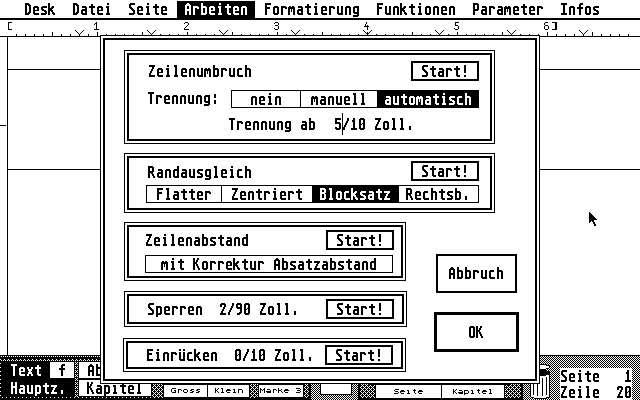
\includegraphics[width=\columnwidth]{img/SNAP4.png}
    \caption{The \textit{Optionen 1...} dialog for text layout}
    \label{fig:text_opts}
\end{figure}

\subsubsection{Accessories \& Tools}

\Signum{} was distributed with a set of additional files that were useful for authoring documents:

\begin{itemize}
    \item Printer \& editor fonts for the character sets \textbf{ANTIKRO}, \textbf{FRAKTUR1}, \textbf{GRAPH1}, \textbf{GRIECH}, \textbf{GROTFE}, \textbf{GROTLT}, \textbf{GROTMIKR}, \textbf{MATHEM}, \textbf{NORMANDE}, and \textbf{PINSEL}.
    \item A set of font editors for the different kinds of printers (\textbf{DCS9N.PRG}, \textbf{DCS24N.PRG} and \textbf{DCS30L.PRG}) as well as a converter from 24-needle printer fonts to laser printer fonts (\textbf{CV24TL30.PRG}).
    \item An \gls{accessory} to capture the current content of the screen to save it as a file that could be loaded into the document (\textbf{SCRCPY.ACC}).
    \item A printer spooler accessory (\textbf{SSP.ACC}) that could improved the printing speed by buffering the output to the actual printer.
    \item A set of printer ''emulators'' that redirected the printer commands to a file (\textbf{PREMUL.PRG}) or to external devices via the serial (\textbf{PEMV24.PRG}), or parallel (\textbf{PEM\_CENT.PRG}) ports.
\end{itemize}

ASH also published a \Signum{} accessory that enabled a right-to-left writing mode, \textbf{SIGREV.ACC}, which proved very useful for scholars that wanted to write Hebrew \cite{stc1988sigrevers}.

\subsection{Fundamentals of File Formats}

A \textit{file format} is a specification that describes how some data is laid out in a \textit{file}, i.e. a sequence of \glspl{byte} that can be saved on a storage device such as a hard disk or flash drive. Most file formats are associated with a file \textit{extension} such as \texttt{*.txt}, \texttt{*.pdf}, \texttt{*.doc} or \texttt{*.png}.

In theory, anyone can specify a file format – either by implementing a software that uses it or by writing a formal specification. In practice, its desirable for software from multiple vendors to use the same, inter-operable file formats.

\subsubsection{Media Types \& Magic Bytes}

To be able to communicate the format of a file without relying on a name or guessing based on the content, the \acrshort{iana} maintains a registry of \glspl{Media Type}\footnote{\url{https://www.iana.org/assignments/media-types/media-types.xhtml}}.

The names listed there are used for downloads and e-mail attachments \cite{rfc6838}. The media types that correspond to the file extensions above are \texttt{text/plain}, \texttt{application/pdf}, \texttt{application/msword}, and \texttt{image/png}.

Some file formats require all \glspl{byte} to be interpreted as characters according to some \gls{encoding}. These are called \textit{text file formats} \cite[§4.2.1]{rfc6838} and should be readable with any plain text editor, for example \textit{Windows Notepad}.

The terms \texttt{ASCII} and \texttt{UTF-8} are used to describe two of the predominant text encoding methods. Formats that include \glspl{byte} that are not encoded as text are usually called \textit{binary file formats}. As the names suggest, files that are stored in a text file format can be edited with a simple text editor, while most binary formats require specialized tools to read or written.

Because file extensions and \acrshort{mime} types are metadata that is not stored in the file itself, most file formats mandate some sort of identifier at the beginning of the file to prevent programs form manipulating a file they were not designed for.

These markers are sometimes called \textit{magic bytes}, presumably because they have no other use than differentiating between formats. For example, a \acrshort{pdf} file always starts with \texttt{\%PDF-} and a \acrshort{png} file with the bytes \fbox{\texttt{89 50 4E 47 0D 0A 1A 0A}}, which contain the string \texttt{PNG}.

\subsubsection{Basic Building Blocks}

This section presents some of the basic building blocks that are used to construct complex file formats. Not all of these apply to the \textit{Signum!} file format, but they should be useful to understand the description in the next section \cite[§1.5]{murray1996eggf}.

\paragraph{Offset \& Format}
There are two aspects that are fundamental to storing a \textit{value} into a file: The first one is the position of that value relative to a reference point or \textit{landmark}. This is called the \textit{offset}. Only two reference points are defined for every file: The \textit{start} and the \textit{end} of the file. %If a format does not require the reference point at the end to start processing, then it's suitable for \textit{streaming}.
The second one is the representation of the data in bytes (or text). This is called the \textit{(binary) format}.

\paragraph{Structures \& Fields}
A \textit{field} is a piece of data that sits at a fixed offset from its reference point. Multiple fields that are stored in sequence starting from a common reference point are collectively called a \textit{struct}.

\paragraph{Arrays \& Streams}
When multiple values of the same kind need to be stored, then they'll usually be stored in sequence. If all values require the same amount of bytes or it's necessary to access one of the elements ''at random'', then every value will be stored at an offset that is a multiple of a known value, the \textit{element length}. This length must be at least as large as the maximum number of bytes that are needed to store one of the values. This whole structure is called an \textit{array}. In some cases, it's useful to store the total length of the array, the element length, or both as a field before the array data to get an array of \textit{variable size}.

Otherwise, when values that would not require the full element length are common or the length is not limited, an element may be stored at next valid offset after the end of the previous one. This is called a \textit{stream} and requires reading all previous elements in order to load a specific one.

\paragraph{Numbers}
On the lowest level of abstraction, all information in a file is stored as numbers. A file is a sequence of \glspl{byte}, each \gls{byte} is made up of 8 \glspl{bit} for a total of 256 different values. In a simple text encoding like ASCII, every character is encoded as one byte value. Sometimes, a byte is subdivided into multiple smaller units, for example 8 units with a value of 0 or 1. This is called a \textit{bitfield}. Sometimes, multiple bytes are grouped to represent a wider range of numbers, e.g. 4 bytes with 32 bits in total, representing 4294967296 distinct values.

\paragraph{Indirect Values}
When the same value is needed multiple times in a file format, it may be useful to store it only once and use a \textit{reference} to that location wherever it is used. One approach to do that is to use the \textit{offset} of the actual value. The other approach is to put these values in an array or stream that is stored somewhere else in the file and use the position in that sequence (the \textit{index}) to represent the value.

\paragraph{Tags}
It's also possible for the structure of the file to depend on the data that is stored. In a format like \LaTeX, a \texttt{\%} sign indicates a comment and \texttt{\textbackslash} indicates a control sequence. In languages like HTML or XML, a \texttt{<} sign indicates a \textit{named tag} and a \texttt{\&} indicates a \textit{named entity}\footnote{Pre-defined text, usually used for writing single characters that are not part of ASCII, e.g. \texttt{euro} for the \euro{} sign}. In other formats, a character code of $0$ is used to mark the end of a string (stream of characters) because it will not appear in any text value. In text formats, it's common for tags to have a matching end tag. A \LaTeX{} comment is terminated by a newline, a HTML named tag is terminated by a \texttt{>} sign and some named tags like \texttt{<a>} require a corresponding closing tag \texttt{</a>}.

\paragraph{Chunks}
Instead of having a dedicated start and end tag, you can also combine a marker with a run-length specifier to specify the bounds of a \textit{chunk}. An early example of a file format using this is the  \acrfull{iff} which uses \acrfullpl{four-cc} to identify file formats and different kinds of parts of the file.

\subsection{Anatomy of a word document}

The Signum!2 document file format uses the file extension \textbf{SDO} and the magic \glspl{byte} are \texttt{sdoc0001}. There is no \textit{Media Type} registered with the IANA for the format.

The general layout of the file format is very similar to and likely inspired by the \acrshort{iff}. The leading \texttt{sdoc} is one example of a \acrshort{four-cc}. Both the \acrshort{iff} \texttt{FORM} format and the \Signum{} file format use a sequence of chunks, saved as pairs of one \acrshort{four-cc} and a 32-bit length specifier followed by a block of data of that length. While \acrshort{iff} files generally use the same chunk type multiple times \cite{amigaos:wordiff}, that is not the case for Signum files. The following subsections present the chunks that it uses in the order that they generally appear in.

One important aspect of this file format is that it is forward- and backward-compatible, that is, newer versions of the software can use files created by older versions and older versions can edit files created by newer versions to some extent without destroying information.

\subsubsection{Header (\texttt{0001})}
\label{sec:sdoc_0001}

The name \textbf{0001} was probably intended to specify the version. This chunk does not contain much data. It does contain information on when the document was created and when it was last saved.

\subsubsection{Character Sets (\texttt{cset})}
\label{sec:sdoc_cset}

The first important section of a Signum! document uses the \textbf{cset} identifier. This section contains an \textit{array} of 8 names with up to 9 characters each. It corresponds to the list of \textit{charsets} that are selected for the document.

Note that the length of the names roughly corresponds to the 8 \gls{byte} limit on file names on the ATARI ST (cf. section 3.1 of \cite{guerin2014filesystem}).

The rest of the file format uses the numbers $0$ through $6$ to represent theses characters sets, so this section is used as a \textit{lookup table} to select the relevant one for a number. In \autoref{fig:cset-dialog}, \textbf{ANTIKRO} would be number $0$, \textbf{NORMANDE} would be number $1$ and \textbf{MATHEM} would be number $2$.

\subsubsection{System Parameters (\texttt{sysp})}
\label{sec:sdoc_sysp}

The next section bears the identifier \textbf{sysp}. At its core, the \Signum{} file format is more of a graphics format than a text format. The parameters correspond to the \textit{Std. Seitenformat} i.e. standard page formatting options in the user interface and are used to set the initial parameters of new pages.

The section also contains additional global configuration such as the settings for automatic page numbering.

\subsubsection{Page Buffer (\texttt{pbuf})}
\label{sec:sdoc_pbuf}

This section (marked \textbf{pbuf}) contains a table with parameters for each page in the document. It starts with the number of pages and the number of \glspl{byte} used for every entry.

Each entry contains an internal index, the logical page number i.e. position within the current document and the physical page number i.e. the position in all documents that make up the final text. It also contains the length of the header and footer as well as the position of the left and right print margin in terms of horizontal coordinates.

\subsubsection{Text Buffer (\texttt{tebu})}
\label{sec:sdoc_tebu}

\begin{figure}[ht]
    \centering
    \begin{Verbatim}[fontsize=\small]
00520c00 40490090 40490005 40490005 .R..@I..@I..@I..
402e0005 4044000b 4049000a 40450005 @...@D..@I..@E..
40520010 40450009 40490009 40430005 @R..@E..@I..@C..
4048000a 4053000b 404b0008 404c000a @H..@S..@K..@L..
407b0008 4053000b 40540008 40450009 @{..@S..@T..@E..
40520009 00120076 0c000045 00979269 @R.....v...E...i
886e9065 8e73a464 90658e72 a2629065 .n.e.s.d.e.r.b.e
8e649065 8e759074 8c658e6e 90738e74 .d.e.u.t.e.n.s.t
8c658e6e a65a9265 8e759067 906e9069 .e.n.Z.e.u.g.n.i
88738e73 8e65a466 8c409072 a2649069 .s.s.e.f.@.r.d.i%
\end{Verbatim}
    \caption{Portion of the text buffer of a document as displayed in a hex-editor. The actual text is supposed to be \foreigntextquote{german}{\underline{III. DIE REICHSKLÖSTER}} and \foreigntextquote{german}{Eines der bedeutensten Zeugnisse für die {[\dots]}} \label{fig:sdo-hexdump}}
\end{figure}

This section uses \textbf{tebu} as its identifier. It is stored as a sequence of chunks that represent the start of a page, the end of a page or a line of characters within a page. Empty lines are not stored. Instead, every line with content starts with a number that specifies how many empty lines were skipped.

The same principle applies within a line: The line is a sequence of character tags that contain the distance from the previous character position, the number of the character set that was used, the number of the character itself and some individual bits that specify which font variants (\ref{sec:font-variants}) were used.

\subsubsection{Hardcopies \& Images (\texttt{hcim})}
\label{sec:sdoc_hcim}

This section is indicated by the \acrshort{four-cc} \textbf{hcim} and contains a sequence of images (hardcopies) that can be used within the document as well as a cross-reference table that defines where parts of the images are actually used.

Because the first version of Signum! did not support images, it's noteworthy that all information related to them is stored in this separate section. This way, an older version of signum can be used to make small changes to the text while keeping this section and thus all images and their position unchanged.

The section starts with a 16 \gls{byte} long header that contains the size in \glspl{byte} of the cross-reference (``site'') table, the number of images and the number of sites.

The header is followed by the site table, which consists of a sequence of 32 \gls{byte} entries that store information like the page, position, height, width and selected area of the original image.

Finally, there is the table of images, which are stored with a filename and encoded according to the \textit{bimc} image file format.

\subsubsection{Unknown sections (\texttt{pl01} \& \texttt{syp2})}
The function of these two chunks is unknown.

\subsection{The \textit{bimc} Image format}

\newcommand{\fboxinclude}[1]{\fbox{\includegraphics[width=0.08\textwidth]{#1}}}
\newcommand{\chk}[1]{\fbox{\makebox(20,20){#1}}}
\newcommand{\chdots}{\makebox(28,26){$\dots$}}
\newcommand{\cvdots}{\makebox(28,26){$\vdots$}}
\newcommand{\cmid}{\makebox(28,26){}}

The \textbf{bimc} file format, specifically version 2 according to the magic \glspl{byte} \textbf{bimc0002}, is a compression scheme for black-and-white images that was used by multiple \gls{ASH} products\footnote{\url{https://www.stcarchiv.de/stm1991/12/piccolo}}.

In the past, there was barely any information publicly available\footnote{\url{https://temlib.org/AtariForumWiki/index.php/Signum!_file_format}} on the details of this format. This is probably due to the fact that \acrshort{ash} products are proprietary and mostly sold to a german audience.

Based on the \textit{68K decompression code} mentioned on that page, I was able to reverse engineer and document the actual compression method.

\subsubsection{Introduction to the compression method}

The \Signum{} handbook \cite[p.~26]{schmerbeck1998signum} explains that a \gls{hardcopy} has the size of an ATARI ST screen i.e. a width of 640 pixels and a height of 400 pixels (\textit{ST-High}). All \textbf{bimc} images that I could find had this size.

\begin{figure}[h]
    \centering
    \chk{$0$} \chk{$1$} \chk{$2$} \chdots \chk{$37$} \chk{$38$} \chk{$39$}\\
    \chk{$40$} \chk{$41$} \chk{$42$} \chdots \chk{$77$} \chk{$78$} \chk{$79$}\\
    \cvdots \cvdots \cvdots \cmid \cvdots \cvdots \cvdots\\
    \chk{$920$} \chk{$921$} \chk{$922$} \chdots \chk{$957$} \chk{$958$} \chk{$959$}\\
    \chk{$960$} \chk{$961$} \chk{$962$} \chdots \chk{$997$} \chk{$998$} \chk{$999$}
    \caption{Position and numbering of chunks in the \textbf{bimc} compression scheme. Every picture has 25 rows and every row has 40 chunks.}
    \label{fig:bimc_chunk_layout}
\end{figure}

The image is partitioned into chunks of 16x16 pixels from left to right, top to bottom i.e. normal English reading order. For the default image size, that is $40 \times 25 = 1000$ chunks in total. Each chunk is further subdivided into four 8x8 sub-chunks: top-left ($A$), top-right ($B$), bottom-left ($C$), and bottom-right ($D$).

\begin{figure}[h]
    \centering
    \chk{$A$} \chk{$B$} \\[1mm]
    \chk{$C$} \chk{$D$}
    \caption{Structure of a chunk in the \textbf{bimc} compression scheme. Each chunk is made up of four $8 \times 8$ pixel sub-chunks.}
    \label{fig:bimc_subchunk_layout}
\end{figure}

It is saved as two sequences: One sequence of bits that we'll call the \textit{control stream} and one sequence of \glspl{byte} that we'll call the \textit{data stream}. In the original, uncompressed image, black is stored as $1$ (\textit{ink}) and white is stored as $0$ (\textit{no ink}).

\paragraph{Concept}
The basic idea of the compression algorithm is only serializing rows-of-chunks, chunks, sub-chunks and rows of pixels in sub-chunks that are non-zero. Additionally, the built-in support for top-to-bottom repetition can switch a lot of the bits to zero if most of the image or most of a chunk uses a plain or checkered background. That last one is useful because a checkered background was commonly used for shades of gray on screens that only supported black and white \cite{toshyp:VDIpatterns}.

\newcommand{\ws}{\square}
\newcommand{\bs}{\blacksquare}
\newcommand{\wbyte}{$\ws\ws\ws\ws\ws\ws\ws\ws$}
\newcommand{\bbyte}{$\bs\bs\bs\bs\bs\bs\bs\bs$}
\newcommand{\wbbyte}{$\ws\bs\ws\bs\ws\bs\ws\bs$}
\newcommand{\bwbyte}{$\bs\ws\bs\ws\bs\ws\bs\ws$}

\paragraph{Note}
The following algorithm uses an operation called \textbf{XOR}. This is short for \textit{Exclusive-Or} because it's identical to using a black pixel if and only if pixels at the same position differ. For example, $\ws\ws\bs\bs \text{ XOR } \ws\bs\bs\ws$ equals $\ws\bs\ws\bs$. Another interpretation is to flip every color (bit) in one operand that is black (set) in the other. Note that the order of the operands does not matter, only that they have the same length.

\subsubsection{Decoding algorithm}

The algorithm to decode and encode images is has two components: The \textit{outer loop} that iterates over the full image and calls a \textit{chunk decoding} algorithm that decodes a single chunk. Decoding requires knowing the width and height of the final image as well as two XOR bytes. These values are provided in the file header.

\paragraph{Outer loop}

\begin{enumerate}
    \item Start with an all-zero (white) image of $600 \times 420$ pixels.
    \item Prepare a 32 \gls{byte} buffer to decode a chunk.
    \item Look at the first row of chunks.
    \item Take one bit from the control stream. If that bit is $0$, skip to step 9.
    \item Otherwise, Look at the first chunk in the current row.
    \item Take one bit from the control stream. If that bit is $0$, skip to step 8.
    \item Decode the chunk using the \textit{chunk decoding} algorithm. Copy the sixteen pairs of \glspl{byte} that represent the sixteen rows of pixels from the buffer to the final image.
    \item Check whether there's another chunk in the same row. If so, move to the next chunk and continue with step 6.
    \item Check whether there's another row in the picture. If so, move to the next row and continue with step 4.
    \item Take the first XOR byte from the header and combine that with every even row of pixels in every sub-chunk.
    \item Finally, take the second XOR byte from the header and combine that with every off row of pixels in every sub-chunk.
\end{enumerate}

\begin{figure}[h]
    \centering
    \fboxinclude{img/bimc-lg/bimc-ex-0-lg.png}%
    \fboxinclude{img/bimc-lg/bimc-ex-1-lg.png}%
    \fboxinclude{img/bimc-lg/bimc-ex-2-lg.png}%
    \fboxinclude{img/bimc-lg/bimc-ex-3-lg.png}%
    \fboxinclude{img/bimc-lg/bimc-ex-4-lg.png}\\[1mm]%
    \fboxinclude{img/bimc-lg/bimc-ex-5-lg.png}%
    \fboxinclude{img/bimc-lg/bimc-ex-6-lg.png}%
    \fboxinclude{img/bimc-lg/bimc-ex-7-lg.png}%
    \fboxinclude{img/bimc-lg/bimc-ex-8-lg.png}%
    \fboxinclude{img/bimc-lg/bimc-ex-9-lg.png}
    \caption{Example of BIMC compressed data. Instead of 32 \glspl{byte} for all 256 pixels, we need only 13 \glspl{byte}. One for every sub-chunk with black pixels and one for every row in a sub-chunk with black pixels}
    \label{fig:bimc_subchunk_data}
\end{figure}

\paragraph{Chunk decoding}
%Recall that every sub-chunk made up of 8 rows that are 8 pixels wide. Starting a $0$, we call rows $0, 2, 4$ and $6$ \textit{even} and rows $1, 3, 5$ and $7$ \textit{odd}.

\begin{enumerate}
    \item Take 2 bits from the control stream. This is the compression mode.
    \item If the bits are $11$ load the next 32 \glspl{byte} from the data stream into the buffer and skip the steps 3 to 7.
    \item Otherwise, take another 4 bits out of the control stream. This is the sub-chunk mask.
    \item If the first bit is set, take one \gls{byte} from the data stream and look at its bits. Every bit corresponds to one of the positions $0, 2, 4, 6, 8, 10, 12, 14$ in the buffer. If it is set, take one \gls{byte} from the data stream and put it in that position. This is the top-left sub-chunk $A$.
    \item Do the same for the second bit of the sub-chunk mask and positions $1, 3, 5, 7, 9, 11, 13, 15$ (top right sub-chunk $B$), the third bit of the sub-chunk mask and positions $16, 18, 20, 22, 24, 26, 28, 30$ (bottom-left sub-chunk $C$), and the fourth bit of the sub-chunk mask and positions $17, 19, 21, 23, 25, 27, 29, 31$. (bottom-right sub-chunk $D$).
    \item Now, recall the compression mode. If the bits are $01$, take \glspl{byte} $0$ and $1$ from the buffer and XOR them with bytes $2$ and $3$. Take the resulting two bytes and XOR them with bytes $4$ and $5$. Repeat that for the complete buffer.
    \item Otherwise, if the compression mode was $10$, take the first four \glspl{byte} ($0$ to $3$ i.e two rows of pixels) and XOR them with \glspl{byte} $4$ through $7$. Take the resulting 4 bytes and XOR them with the next four. Repeat that for the rest of the buffer.
\end{enumerate}

Done!

\begin{figure}[h]
    \centering
    \fboxinclude{img/bimc-lg/bimc-ex-9-lg.png}$\to$%
    \fboxinclude{img/bimc-lg/bimc-ex-10-lg.png}$\to$%
    \fboxinclude{img/bimc-lg/bimc-ex-11-lg.png}$\to$%
    \fboxinclude{img/bimc-lg/bimc-ex-12-lg.png}\\[2mm]$\to$%
    \fboxinclude{img/bimc-lg/bimc-ex-13-lg.png}$\to$%
    \fboxinclude{img/bimc-lg/bimc-ex-14-lg.png}$\to$%
    \fboxinclude{img/bimc-lg/bimc-ex-15-lg.png}$\to$%
    \fboxinclude{img/bimc-lg/bimc-ex-16-lg.png}
    \caption{Example of the final step of decoding a chunk that was compressed with strategy 2. \label{fig:bimc_chunk_xor}}
\end{figure}

%\subsubsection{Encoding algorithm}
%
%The encoding algorithm is the same procedure just in reverse. The main challenge in writing the encoder is to choose a good compression mode for each chunk and good final XOR bytes without taking too much time analyzing the uncompressed image. The following algorithm proposes methods to achieve this but actual implementations may choose a different approach. We call a row, chunk, sub-chunk or row of a sub-chunk \textit{non-white} if at least one of its pixels is black.
%
%\paragraph{Outer loop}
%
%\begin{enumerate}
%    \item For every even row in every sub-chunk, find the pattern
%    that is most common. Let's call that pattern $X_A$. Do the same for every odd row in every odd sub-chunk and call that $X_B$. For an image that is predominantly white, both will be \wbyte. For an image that is predominantly black, both will be \bbyte. For an image that is predominantly checkered, one might be \bwbyte~while the other is \wbbyte.
%    \item Now, for every even row in every sub-chunk, flip every pixel that is black in $X_A$. Do the same for every odd row in every sub-chunk but with $X_B$. This has the effect that the most common row is \wbyte~now.
%    \item Now, start on the first row of chunks
%    \item If the complete row is white, write a $0$ to the control stream and skip to step 9
%    \item Otherwise, look at the first chunk in the row
%    \item If the complete chunk is white, write a $0$ to the control stream and skip to step 8
%    \item Encode the chunk using the \textit{chunk encoding} algorithm.
%    \item Check whether there's another chunk in the same row. If so, move to the next chunk and continue with step 6.
%    \item Check whether there's another row in the picture. If so, move to the next row and continue with step 4.
%    \item Save the file and store $X_A$ and $X_B$ in its header.
%\end{enumerate}
%
%\paragraph{Chunk encoding}
%
%\begin{enumerate}
%    \item Count the number of sub-chunks that are not completely white plus the total number of non-white rows in these sub-chunks. We'll call that $c_0$.
%    \item Then, count the number of sub-chunks and rows that are non-white when every row (except the first) is XOR-ed with the row directly above. We'll call that $c_1$.
%    \item Then, count the number of sub-chunks and rows that are non-white when every row (except the first two) is XOR-ed with the row two above them. We'll call that $c_2$.
%    \item Finally, set $c_3$ to $32$. Each value $c_x$ represents the number of bytes that are written for one of the compression modes $x \in {0, 1, 2, 3}$.
%    \item Now, choose the compression mode $x$ with the minimal value for $c_x$. If that minimum is $32$, choose mode $3$. Write the compression mode to the control stream as a 2-bit binary number.
%    \item If the compression mode is $3$, write the complete buffer to the data stream and skip the last two steps.
%    \item Otherwise, apply the XOR-operations for modes $1$ and $2$.
%    \item Then, for every sub-chunk ($A,B,C,D$), write $0$ to the control stream if the sub-chunk is completely white. Otherwise, write $1$ to the control stream and one \gls{byte} to the data stream where each indicates whether the corresponding row is non-white. Then, write those non-white row in the sub-chunk to the data stream.
%\end{enumerate}
%
%Done!
\section{A modern re-implementation}

There are three main forms in which Signum documents still exist today: printed, stored in the original file format or exported as plain text \cite{xchem2001atari}.

In print, the text is readable but any possibility of editing the document in the future is lost. In the original format, no information is lost but using it requires running the original software, which is only available for a discontinued operating system. In plain text, the character order is preserved, but graphical features like images, formulas or foreign language fonts are lost.

The apparent solution is to take the original format, which has all relevant information still intact, and convert it into a format that can be used with modern tools.

Thus, based on the knowledge I derived from experiments with running Signum! in an emulator (cf. \autoref{sec:emulator}), the few pieces of code working with these file formats that I found on the internet and reading the \textit{Das Signum! Buch} \cite{ritzhaupt1988signum}, I implemented a software that is able to read, process and convert Signum!2 documents.

This software is available for others to use and is implemented using the Rust programming language \cite{xipho2020sdotool}.

\subsection{Using the Rust programming language}

Rust is a systems programming language that presents itself with the tagline \textit{A language empowering everyone to build reliable and efficient software}\footnote{\url{https://rust-lang.org}}. It comes with a package manager called \textit{Cargo} and built-in capabilities for dependency management, automatic tests, generating documentation from code and comments and a large standard library of utilities.

Initially developed as a hobby project, it was adopted as a research project by \textit{Mozilla} in 2010 and released to a wider audience in 2015. Starting out from the position to \textquote{Concentrate on known ways of achieving more safety, more concurrency, less mess} \cites{rustNothingNew, rustRefInfluences}, it has since been adopted at all of the big 5 tech companies (Google, Apple, Facebook, Amazon, Microsoft) and has recently established its own foundation \cite{mzla2021rustfoundation}.

Using Rust, I could build on top of existing libraries, such as \textit{nom} for parsing file formats and \textit{image} for encoding images to modern formats, just by adding their name to a list of dependencies \cites{geal2020nom, rs2020image}. In the same spirit, I have released reusable components of my work to that same package registry \cites{xipho2021signum, xipho2020pdfc, xipho2020ccitt}.

Rust is also useful in this case, because the language makes it easy to write correct code by modeling edge cases in data types. There is no special \texttt{null} value that indicates the absence of a value. If a value of type \texttt{T} may not be available, then the type of that value is \texttt{Option<T>} and, which must be \textit{unwrapped} before accessing the inner value. A program always halts with a useful error message by default if a problem is encountered.

Finally, it's normal for errors to occur in the case of reverse engineering a file format. Using a languages that provides a reasonable certainty that the code does what is intended, if it compiles successfully, implies that the error is most likely caused by a misunderstanding of the file format and not by a mistake in the implementation.

\subsection{PostScript / PDF}

Ever since the ATARI and Signum! were discontinued, users of the software
were interested in exporting their documents for use in other systems. While there are recommendations on how to do just that, all of them have their own limitations.

Commonly, the request was to be able to open Signum! files with other word processing programs like \textit{StarOffice} or \textit{MS Word}. In this section, I'll explain why I focused my attention on PDF as an output format instead.

\subsubsection{Conversion to modern formats}

Today, the Signum! file format is no longer in use. The only software that could read it was only available on the the ATARI ST. There was a conversion software (\textbf{TEXTCONV.PRG}) packaged with another word processor for the ATARI called \textit{Papyrus}, which could export to \acrfull{rtf}. However, the result isn't great for anything that isn't plain text.

Signum! itself had the ability to export to ASCII, which also lacked all of the advanced formatting options. The next version, Signum!3 could also read the files from the previous version but it comes with its own custom file format that no other programs support.

The third strategy was to use a virtual printer to print Signum! documents to a set of images instead of paper on a real printer. This had the advantage of preserving the documents at a very high quality and accuracy. The downside is that, even with subsequent processing using \textit{Optical Character Recognition}, it's prone to errors and hard to search or re-use the text.

\subsubsection{A page definition language}

As explained in \autoref{sec:sdoc_tebu}, Signum documents store their text based on the position of the characters, not their order in the text. An expression like $Q_2$ would be typeset as a $Q$ on one line and a small $2$ on a line further down. To turn this into a tag based document language like \acrshort{html} or \textit{MS Word 2007 (docx)} requires interpreting these relationships.

Ideally, these positions could just be re-used in the new format. The relevant goal is keeping information about the characters so that the text is searchable. The text alone does not have contain information to produce an accurate copy of the original. This is exactly what a \acrfull{pdl} is used for.

\textit{PostScript} is a programming language crated by \textit{Adobe} and is most commonly used as a \acrlong{pdl}. It provides built-in commands like \texttt{moveto} and \texttt{setfont} that manipulate a graphics model that is ultimately sent to an output device with the \texttt{showpage} command.

\textit{\acrshort{pdf}} is a file format also created by \textit{Adobe} that is based on PostScript. The main difference is that PDF is a structured container format that mandates pages and fonts to be specified in a certain way at a pre-defined location, it only provides a subset of all PostScript commands and uses shorter names for them.

So, to translate a \Signum{} file, the approach I chose was to place every character in the correct position independent of all other characters and to gradually introduce logic that removes unnecessary commands. Examples for the latter would be zero-length moves between adjacent characters or switching to the font that's currently active.

\subsection{Bitmap Fonts}

Another challenge in recreating Signum! documents in modern formats were the fonts. As mentioned earlier, it used a set of custom file formats that contained the glyphs for each character in a charset depending on the output device.

Fonts are typically crated as \textit{outlines} by a company called a \textit{font foundry}. These outlines are then \textit{rasterized} at different sizes, that is converted into a format that specifies which positions on a paper or display should be coloured.

One description of this process for a commercial typewriter of the 1980s can be found in a memo by employees of \textit{Bell Labs} \cite[Page 7]{bwk1980summer}, which was the research \& development department of US-American telephone company AT\&T well-known for the development of the UNIX operating system.

These intermediary file formats are called \textit{bitmap fonts} and contain little pixel images for every character or ligature in the font. Both the ATARI ST and the X11 window system first released in 1984 used bitmap fonts initially \cite{tosVDIfontHdr} \cite{ffPCFFormat}.

\begin{figure}
    \centering
    \fbox{\begin{varwidth}{\textwidth}
    $\bs\bs\bs\bs\bs\bs\bs\bs\bs\bs\bs\bs\bs\bs\bs\bs\bs\bs\bs$\\[-1mm]%
    $\bs\bs\bs\bs\bs\bs\bs\bs\bs\bs\bs\bs\bs\bs\bs\bs\bs\bs\bs$\\[-1mm]%
    $\ws\ws\ws\bs\bs\bs\bs\bs\bs\ws\ws\ws\ws\ws\ws\ws\bs\bs\bs$\\[-1mm]%
    $\ws\ws\ws\bs\bs\bs\bs\bs\bs\ws\ws\ws\ws\ws\ws\ws\bs\bs\bs$\\[-1mm]%
    $\ws\ws\ws\bs\bs\bs\bs\bs\bs\ws\ws\ws\ws\ws\ws\ws\bs\bs\bs$\\[-1mm]%
    $\ws\ws\ws\bs\bs\bs\bs\bs\bs\ws\ws\ws\ws\ws\ws\ws\bs\bs\bs$\\[-1mm]%
    $\ws\ws\ws\bs\bs\bs\bs\bs\bs\ws\ws\ws\ws\ws\ws\ws\ws\ws\ws$\\[-1mm]%
    $\ws\ws\ws\bs\bs\bs\bs\bs\bs\ws\ws\ws\ws\bs\bs\bs\ws\ws\ws$\\[-1mm]%
    $\ws\ws\ws\bs\bs\bs\bs\bs\bs\ws\ws\ws\ws\bs\bs\bs\ws\ws\ws$\\[-1mm]%
    $\ws\ws\ws\bs\bs\bs\bs\bs\bs\ws\ws\ws\ws\bs\bs\bs\ws\ws\ws$\\[-1mm]%
    $\ws\ws\ws\bs\bs\bs\bs\bs\bs\bs\bs\bs\bs\bs\bs\bs\ws\ws\ws$\\[-1mm]%
    $\ws\ws\ws\bs\bs\bs\bs\bs\bs\bs\bs\bs\bs\bs\bs\bs\ws\ws\ws$\\[-1mm]%
    $\ws\ws\ws\bs\bs\bs\bs\bs\bs\ws\ws\ws\ws\bs\bs\bs\ws\ws\ws$\\[-1mm]%
    $\ws\ws\ws\bs\bs\bs\bs\bs\bs\ws\ws\ws\ws\bs\bs\bs\ws\ws\ws$\\[-1mm]%
    $\ws\ws\ws\bs\bs\bs\bs\bs\bs\ws\ws\ws\ws\bs\bs\bs\ws\ws\ws$\\[-1mm]%
    $\ws\ws\ws\bs\bs\bs\bs\bs\bs\ws\ws\ws\ws\ws\ws\ws\ws\ws\ws$\\[-1mm]%
    $\ws\ws\ws\bs\bs\bs\bs\bs\bs\ws\ws\ws\ws\ws\ws\ws\ws\bs\bs$\\[-1mm]%
    $\ws\ws\ws\bs\bs\bs\bs\bs\bs\ws\ws\ws\ws\ws\ws\ws\ws\bs\bs$\\[-1mm]%
    $\ws\ws\ws\bs\bs\bs\bs\bs\bs\ws\ws\ws\ws\ws\ws\ws\ws\bs\bs$\\[-1mm]%
    $\ws\ws\ws\bs\bs\bs\bs\bs\bs\ws\ws\ws\ws\ws\ws\ws\ws\bs\bs$\\[-1mm]%
    $\bs\bs\bs\bs\bs\bs\bs\bs\bs\bs\bs\bs\bs\bs\bs\bs\bs\bs\bs$\\[-1mm]%
    $\bs\bs\bs\bs\bs\bs\bs\bs\bs\bs\bs\bs\bs\bs\bs\bs\bs\bs\bs$
    \end{varwidth}}
    \caption{A pixel image for the letter \textbf{\fontfamily{bch} \selectfont E} in the \textit{Bitstream Charter} font in bold at size $24$. \label{fig:bitmap_letter}}
\end{figure}

The first step of my work on \Signum fonts was to figure out the layout of the \textbf{E24}, \textbf{P24} and \textbf{L30} font files and find the pixel images for every character. Fortunately, letters are relatively easy to find when looking at the binary representation of a file. There are usually far fewer alternations between zeroes and ones i.e. black and white in bitmaps that in numeric data.

\subsubsection{TeX + Metafont}

The \TeX{} typesetting system was released in 1986 with the goal of producing documents of \textit{the best} quality. One way that the author, Donald Knuth, intended to achieve this was by creating a program called \textbf{METAFONT} that would take a outline description of the characters of a font and translate them into bitmap fonts of the correct resolution on demand when a \TeX{} document was compiled.

Originally, \TeX{} documents were turned into a format called \textbf{DVI} (\textit{device-independent}) before being sent to a printer. Most modern users of \LaTeX{} use the \texttt{pdflatex} program, which turns \TeX{} files directly into \acrshortpl{pdf}. But it is still possible to use the original toolchain.

The program \texttt{latex} turns a \TeX{} file that uses \LaTeX{} macros (e.g. \texttt{\textbackslash documentclass}) into a \texttt{*.dvi} file. The program \texttt{dvips} turns the DVI file into a \textit{PostScript} program and a PostScript interpreter like \textit{Adobe Distiller} or \textit{GhostScript} turns that program into a PDF file.

It's possible to tell \texttt{dvips} to embed the bitmap fonts generated by METAFONT into the PostScript program. By reverse-engineering how that embedding works, I could substitute the bitmaps that I extracted from the \Signum{} fonts. Ultimately, this is the opposite of what people commonly want\footnote{\url{http://www.texfaq.org/FAQ-pkfix}} and the end result is a standard \textit{Adobe Type3} font.

As with a lot of this project, my first priority was to produce something that produces a recognizable result, then improve my understanding of how it works and eventually replace parts of the system with technologies that are better suited for the task at hand.

\subsubsection{Ghostscript and CCITTFaxDecode}

With the ability to transform \Signum{} texts into PostScript programs, the next step was to compile these programs into PDFs using \textit{Ghostscript} and understanding the way that text and fonts were encoded there.

The fonts were still stored as Adobe Type3 but this time, the individual pixel images for the glyphs were encoded by an algorithm called \textit{\acrshort{ccitt}FaxDecode}. That is the name PDF uses to refer to \textit{International Telecommunications Union (ITU), Recommendations T.4 and T.6} \cites{murray1996ccitt, ccitt1988t4, ccitt1988t6}, originally published in November of 1988.

These algorithms were specifically developed to be good at compressing text documents for use in fax machines. They work particularly well for documents that have a small number of changes between black and white on every line of pixels and which don't change much from one such line to the next.

To be able to use this compression for \Signum{} fonts, I created a \acrshort{ccitt} Group 4 2-Dimensional encoder and a decoder in Rust and made them publicly available\footnote{\url{https://xiphoseer.github.io/sdo-tool/implementation\#ccitt-t4-t6}}.

% (maybe TROFF)
\label{sec:encoding}
\subsection{Font Encoding}

The final challenge related to \Signum{} fonts was to determine which characters were actually provided as part of a charset. A person can look at the bitmap of character number 65 of the \textbf{ANTIKRO} charset and decide that it is the letter \textit{A}, but that involves a lot more work for an automatic system.

Fortunately, the mapping of numbers to keys on the ATARI keyboard is always the same, so all fonts that were just visual variations of these same characters used the same standard mapping\footnote{\href{https://github.com/Xiphoseer/sdo-tool/blob/196fbf9e79c127cb6bfda1a5bb91e51581d050b1/crates/sdo-pdf/src/font.rs\#L20-L44}{Xiphoseer/sdo-tool:/crates/sdo-pdf/src/font.rs\#L20-L44}}. This standard is mostly consistent with the printable characters in the \textit{American Standard Code for Information Interchange (ASCII)}, one of the foundational standards in computing. However, the \Signum{} encoding uses the numbers $1$ to $31$, which are assigned to non-printable control codes in ASCII, for characters typed in using the numpad.

\begin{figure}[h]
    \centering
    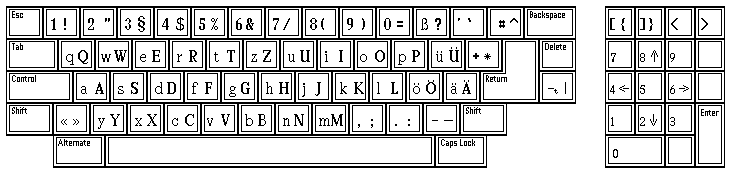
\includegraphics[width=\columnwidth]{img/ANTIKRO.png}
    \caption{The document \textbf{KBANTIK.SDO} that is distributed with \Signum{}. It provides a visual reference to determine which physical key corresponds to which character number, independent of the current character set}
    \label{fig:my_label}
\end{figure}

The computing industry has since created the \gls{Unicode} standard, which aims to assign a single number called a \gls{codepoint} to every character that is used in any amount of significant documents written in a current or historic language\funfact{This occasionally has unintentional side-effects like adopting Emoji worldwide when integrating the japan-specific \textit{ShiftJIS} encoding\href{https://www.theverge.com/2013/3/4/3966140/how-emoji-conquered-the-world}{$[A]$}\href{https://www.youtube.com/watch?v=5OPkGQoPeHk}{$[B]$}}.

This is useful to solve the same kind of challenges that \Signum{} was used for: Writing mixed-language text with built-in support for languages like Greek or Hebrew.

\gls{Unicode} uses \textit{mapping tables} to describe the transformation of one text encoding into \glspl{codepoint} \cite{unicode2015atarist}. As every \Signum{} charset can represent an encoding as well as a font, it's possible to create mapping files for some of the charsets \cite{xipho2020antikro} and re-use them for other character sets which match the same encoding.
\section*{Conclusion}
\label{sec:conclusion}
\addcontentsline{toc}{section}{\nameref{sec:conclusion}}

Working to restore a document file format requires a lot of knowledge in related domains. This project allowed me to learn more about operating systems, fonts, text encoding, page definition languages, and image compression.

My initial motivation for this project was a box with floppy disks that my parents used about 25 to 30 years ago. I've known for a while that one of the disks likely contained my fathers masters thesis (\textit{Magister Artium}) and that it was written in Signum, but my understanding of legacy computer systems was not sufficient at the time when I first learned about it.

At this point, the project has progressed far enough that I can take the thesis files which I extracted from one of the floppy disks, run them through my system and get a searchable PDF out of it. I've also been in contact with a small number of people that did not have such a tool available to them and graciously supported the project by sending me their original documents.

% - Make this possible for others
I suspect that there are still a number of printed theses sitting in German university libraries whose authors still have the original Signum! files and which could be digitized using my tool, but I think it would be very difficult to identify even a small group of them.

%From contacting the person that created \textbf{TEXTCONV.PRG}, I know that a lot of people needed and received help with recovering Signum files around the year 2000. 

% - Outlook: Can be useful to learn from something that was there instead of reinventing the wheel. ref: rust -> TWIR
Finally, I think that \Signum{} is a good example for why it can be useful to learn from something that was created in the past, rather than inventing a new systems. To this day, there are students discussing whether \LaTeX or Microsoft word are more appropriate for homework in university classes. The ''best'' method would probably be a mixture of the two systems but for all practical purposes, the answer is to use whatever fits best to the author and their, possibly non-standard, requirements.

\subsection*{Future Work}
\label{subsec:conclusion}
\addcontentsline{toc}{subsection}{\nameref{subsec:conclusion}}

While this paper is now complete, there is a lot more that I want to achieve in terms of tools related to \Signum{}:

Firstly, I want to continue the work on the tool that exports documents to PDF and add support for Unicode encoding (\ref{sec:encoding}) to the fonts that are embedded into the output files. This requires creating and loading mapping files for each character set.

Then, I want to create a tool that allows the creation of Unicode mapping files with a graphical user interface. The end goal is to have a tool that presents one character after the other and the default encoding for that character and asks the user to confirm the encoding, type in the correct Unicode code-point or mark the character as missing.

I want to investigate converting \Signum{} fonts into \textit{OpenType} fonts, or any other font format that would work on the web. The goal here is to have fonts available that have the same dimensions as the originals and can be used in contexts where I don't control the font rendering.

Next, I want to create a tool that turns \Signum{} documents into web pages. This works best, if the previous tasks are already complete, but may work reasonably well for simple documents.

Finally, I want to investigate the \textit{ESC/P} instructions that \Signum{} sends to printers to get a better understanding of how it manipulates character bitmaps to produce bold, italic, wide, tall and short font variants (\ref{sec:font-variants}).

{\scriptsize
I want to thank the author, Franz Schmerbeck, for creating this program; Volker Ritzhaupt and Oliver Buchmann of ASH for publishing it, providing support to original users and co-authoring the handbook \cite{schmerbeck1998signum} and the user guide \cite{ritzhaupt1988signum}; Lonny Pursell for helping me find a working image decompression program; Thomas Tempelmann for uploading example files with images and other people that I've reached out to over the course of this project.}

\printglossary[type=\acronymtype]
\printglossary
\listoffigures
\printbibliography
%\printurls
\checkproblems
\end{document}
